\documentclass[twoside]{book}

% Packages required by doxygen
\usepackage{fixltx2e}
\usepackage{calc}
\usepackage{doxygen}
\usepackage[export]{adjustbox} % also loads graphicx
\usepackage{graphicx}
\usepackage[utf8]{inputenc}
\usepackage{makeidx}
\usepackage{multicol}
\usepackage{multirow}
\PassOptionsToPackage{warn}{textcomp}
\usepackage{textcomp}
\usepackage[nointegrals]{wasysym}
\usepackage[table]{xcolor}

% Font selection
\usepackage[T1]{fontenc}
\usepackage[scaled=.90]{helvet}
\usepackage{courier}
\usepackage{amssymb}
\usepackage{sectsty}
\renewcommand{\familydefault}{\sfdefault}
\allsectionsfont{%
  \fontseries{bc}\selectfont%
  \color{darkgray}%
}
\renewcommand{\DoxyLabelFont}{%
  \fontseries{bc}\selectfont%
  \color{darkgray}%
}
\newcommand{\+}{\discretionary{\mbox{\scriptsize$\hookleftarrow$}}{}{}}

% Page & text layout
\usepackage{geometry}
\geometry{%
  a4paper,%
  top=2.5cm,%
  bottom=2.5cm,%
  left=2.5cm,%
  right=2.5cm%
}
\tolerance=750
\hfuzz=15pt
\hbadness=750
\setlength{\emergencystretch}{15pt}
\setlength{\parindent}{0cm}
\setlength{\parskip}{3ex plus 2ex minus 2ex}
\makeatletter
\renewcommand{\paragraph}{%
  \@startsection{paragraph}{4}{0ex}{-1.0ex}{1.0ex}{%
    \normalfont\normalsize\bfseries\SS@parafont%
  }%
}
\renewcommand{\subparagraph}{%
  \@startsection{subparagraph}{5}{0ex}{-1.0ex}{1.0ex}{%
    \normalfont\normalsize\bfseries\SS@subparafont%
  }%
}
\makeatother

% Headers & footers
\usepackage{fancyhdr}
\pagestyle{fancyplain}
\fancyhead[LE]{\fancyplain{}{\bfseries\thepage}}
\fancyhead[CE]{\fancyplain{}{}}
\fancyhead[RE]{\fancyplain{}{\bfseries\leftmark}}
\fancyhead[LO]{\fancyplain{}{\bfseries\rightmark}}
\fancyhead[CO]{\fancyplain{}{}}
\fancyhead[RO]{\fancyplain{}{\bfseries\thepage}}
\fancyfoot[LE]{\fancyplain{}{}}
\fancyfoot[CE]{\fancyplain{}{}}
\fancyfoot[RE]{\fancyplain{}{\bfseries\scriptsize Generated by Doxygen }}
\fancyfoot[LO]{\fancyplain{}{\bfseries\scriptsize Generated by Doxygen }}
\fancyfoot[CO]{\fancyplain{}{}}
\fancyfoot[RO]{\fancyplain{}{}}
\renewcommand{\footrulewidth}{0.4pt}
\renewcommand{\chaptermark}[1]{%
  \markboth{#1}{}%
}
\renewcommand{\sectionmark}[1]{%
  \markright{\thesection\ #1}%
}

% Indices & bibliography
\usepackage{natbib}
\usepackage[titles]{tocloft}
\setcounter{tocdepth}{3}
\setcounter{secnumdepth}{5}
\makeindex

% Custom commands
\newcommand{\clearemptydoublepage}{%
  \newpage{\pagestyle{empty}\cleardoublepage}%
}

\usepackage{caption}
\captionsetup{labelsep=space,justification=centering,font={bf},singlelinecheck=off,skip=4pt,position=top}

%===== C O N T E N T S =====

\begin{document}

% Titlepage & ToC
\pagenumbering{alph}
\begin{titlepage}
\vspace*{7cm}
\begin{center}%
{\Large Proyecto 1 }\\
\vspace*{1cm}
{\large Generated by Doxygen 1.8.13}\\
\end{center}
\end{titlepage}
\clearemptydoublepage
\pagenumbering{roman}
\tableofcontents
\clearemptydoublepage
\pagenumbering{arabic}

%--- Begin generated contents ---
\chapter{Class Index}
\section{Class List}
Here are the classes, structs, unions and interfaces with brief descriptions\+:\begin{DoxyCompactList}
\item\contentsline{section}{\hyperlink{classblastobject}{blastobject} }{\pageref{classblastobject}}{}
\end{DoxyCompactList}

\chapter{File Index}
\section{File List}
Here is a list of all documented files with brief descriptions\+:\begin{DoxyCompactList}
\item\contentsline{section}{{\bfseries blastobject.\+h} }{\pageref{blastobject_8h}}{}
\item\contentsline{section}{\hyperlink{main_8cpp}{main.\+cpp} \\*En este programa se utiliza el algoritmo B\+L\+A\+ST para comparacion de secuencias en su version mas simple, comparando con una base de datos creada por el usuario con el proposito de observar su comportamiento de algoritmo y sus resultados. En este caso dichos objetos son del tipo blastobject }{\pageref{main_8cpp}}{}
\end{DoxyCompactList}

\chapter{Class Documentation}
\hypertarget{classblastobject}{}\section{blastobject Class Reference}
\label{classblastobject}\index{blastobject@{blastobject}}
\subsection*{Public Member Functions}
\begin{DoxyCompactItemize}
\item 
\hypertarget{classblastobject_a1ed96bf0cf72600743a56b37ae6e0c16}{}\label{classblastobject_a1ed96bf0cf72600743a56b37ae6e0c16} 
\hyperlink{classblastobject_a1ed96bf0cf72600743a56b37ae6e0c16}{blastobject} ()
\begin{DoxyCompactList}\small\item\em Constructor vacio de clase blastobject. \end{DoxyCompactList}\item 
\hyperlink{classblastobject_aa6004c11726327285515febd40f26b28}{blastobject} (const \hyperlink{classblastobject}{blastobject} \&orig)
\begin{DoxyCompactList}\small\item\em Constructor de la clase blastobject. \end{DoxyCompactList}\item 
\hypertarget{classblastobject_a5dcb3ba619d57005aa6ed2169fcbf5c3}{}\label{classblastobject_a5dcb3ba619d57005aa6ed2169fcbf5c3} 
virtual \hyperlink{classblastobject_a5dcb3ba619d57005aa6ed2169fcbf5c3}{$\sim$blastobject} ()
\begin{DoxyCompactList}\small\item\em Destructor de la clase blastobject. \end{DoxyCompactList}\item 
char \hyperlink{classblastobject_aeb5a23c8caddb226fa161fe3cb162c23}{comparador} (char $\ast$$\ast$lista, int contador)
\begin{DoxyCompactList}\small\item\em Compara las secuencias de caracteres con la tabla de traduccion. \end{DoxyCompactList}\item 
int \hyperlink{classblastobject_a50f753f559096d95d75ee73ae08b846e}{gapclear} (char $\ast$$\ast$lista)
\begin{DoxyCompactList}\small\item\em Retorna una secuencia con solo los caracteres similares. \end{DoxyCompactList}\item 
int \hyperlink{classblastobject_a0426c755487823aebf8734b19e668a49}{raw} (char $\ast$$\ast$lista)
\begin{DoxyCompactList}\small\item\em Compara las secuencias de caracteres con la referencia y cuenta su puntuacion cruda. \end{DoxyCompactList}\item 
int \hyperlink{classblastobject_ae6ca5436041b743e8c20739a9f59ef91}{gap} (char $\ast$$\ast$lista, int n)
\begin{DoxyCompactList}\small\item\em Compara las secuencias de caracteres con la referencia y cuenta sus vacios. \end{DoxyCompactList}\end{DoxyCompactItemize}
\subsection*{Public Attributes}
\begin{DoxyCompactItemize}
\item 
\hypertarget{classblastobject_ad9bd5756d99478be4072818bffa2bc9e}{}\label{classblastobject_ad9bd5756d99478be4072818bffa2bc9e} 
int {\bfseries rawscore}
\item 
\hypertarget{classblastobject_afc851d8c3cf8495abf28c707e5c28fed}{}\label{classblastobject_afc851d8c3cf8495abf28c707e5c28fed} 
int {\bfseries gapcounter}
\item 
\hypertarget{classblastobject_a801149f5f021420528a7f2b593f9c7f0}{}\label{classblastobject_a801149f5f021420528a7f2b593f9c7f0} 
int {\bfseries size}
\item 
\hypertarget{classblastobject_adc4e3120d055bdd7e2ec1cb704796fdb}{}\label{classblastobject_adc4e3120d055bdd7e2ec1cb704796fdb} 
const char $\ast$ {\bfseries base}
\end{DoxyCompactItemize}


\subsection{Constructor \& Destructor Documentation}
\hypertarget{classblastobject_aa6004c11726327285515febd40f26b28}{}\label{classblastobject_aa6004c11726327285515febd40f26b28} 
\index{blastobject@{blastobject}!blastobject@{blastobject}}
\index{blastobject@{blastobject}!blastobject@{blastobject}}
\subsubsection{\texorpdfstring{blastobject()}{blastobject()}}
{\ttfamily blastobject\+::blastobject (\begin{DoxyParamCaption}\item[{const \hyperlink{classblastobject}{blastobject} \&}]{orig }\end{DoxyParamCaption})}



Constructor de la clase blastobject. 


\begin{DoxyParams}{Parameters}
{\em blastobject\&} & Constante objeto. \\
\hline
\end{DoxyParams}


\subsection{Member Function Documentation}
\hypertarget{classblastobject_aeb5a23c8caddb226fa161fe3cb162c23}{}\label{classblastobject_aeb5a23c8caddb226fa161fe3cb162c23} 
\index{blastobject@{blastobject}!comparador@{comparador}}
\index{comparador@{comparador}!blastobject@{blastobject}}
\subsubsection{\texorpdfstring{comparador()}{comparador()}}
{\ttfamily char blastobject\+::comparador (\begin{DoxyParamCaption}\item[{char $\ast$$\ast$}]{lista,  }\item[{int}]{contador }\end{DoxyParamCaption})}



Compara las secuencias de caracteres con la tabla de traduccion. 

La funcion recorre el arreglo ingresado para luego regresar la evaluacion correspondiente a la comparacion realizada.


\begin{DoxyParams}{Parameters}
{\em lista} & Secuencia de caracteres ingresados por el usuario. \\
\hline
{\em contador} & Variable de control para el contador que recorre el arreglo \\
\hline
\end{DoxyParams}
\begin{DoxyWarning}{Warning}
El primer dato de la lista es el nombre del ejecutable. 
\end{DoxyWarning}
\hypertarget{classblastobject_ae6ca5436041b743e8c20739a9f59ef91}{}\label{classblastobject_ae6ca5436041b743e8c20739a9f59ef91} 
\index{blastobject@{blastobject}!gap@{gap}}
\index{gap@{gap}!blastobject@{blastobject}}
\subsubsection{\texorpdfstring{gap()}{gap()}}
{\ttfamily int blastobject\+::gap (\begin{DoxyParamCaption}\item[{char $\ast$$\ast$}]{lista,  }\item[{int}]{n }\end{DoxyParamCaption})}



Compara las secuencias de caracteres con la referencia y cuenta sus vacios. 

La funcion recorre el arreglo ingresado para luego regresar la evaluacion correspondiente a la cantidad de vacios existentes en la secuencia comparada.


\begin{DoxyParams}{Parameters}
{\em lista} & Secuencia de caracteres ingresados por el usuario. \\
\hline
{\em n} & Variable de control para la cantidad de pasos de recorrido. \\
\hline
\end{DoxyParams}
\begin{DoxyWarning}{Warning}
El primer dato de la lista es el nombre del ejecutable. 
\end{DoxyWarning}
Here is the call graph for this function\+:
\nopagebreak
\begin{figure}[H]
\begin{center}
\leavevmode
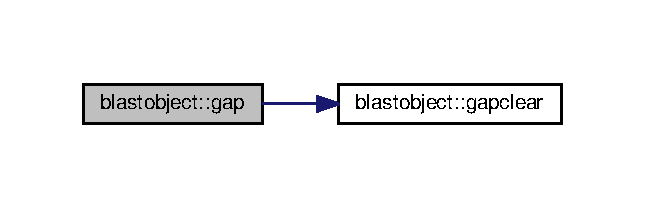
\includegraphics[width=310pt]{classblastobject_ae6ca5436041b743e8c20739a9f59ef91_cgraph}
\end{center}
\end{figure}
\hypertarget{classblastobject_a50f753f559096d95d75ee73ae08b846e}{}\label{classblastobject_a50f753f559096d95d75ee73ae08b846e} 
\index{blastobject@{blastobject}!gapclear@{gapclear}}
\index{gapclear@{gapclear}!blastobject@{blastobject}}
\subsubsection{\texorpdfstring{gapclear()}{gapclear()}}
{\ttfamily int blastobject\+::gapclear (\begin{DoxyParamCaption}\item[{char $\ast$$\ast$}]{lista }\end{DoxyParamCaption})}



Retorna una secuencia con solo los caracteres similares. 

La funcion recorre el arreglo ingresado para luego imprimir la secuencia con los caracteres similares y los vacios rellenos con el simbolo de suma +.


\begin{DoxyParams}{Parameters}
{\em lista} & Secuencia de caracteres ingresados por el usuario. \\
\hline
\end{DoxyParams}
\begin{DoxyWarning}{Warning}
El primer dato de la lista es el nombre del ejecutable. 
\end{DoxyWarning}
Here is the caller graph for this function\+:
\nopagebreak
\begin{figure}[H]
\begin{center}
\leavevmode
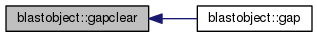
\includegraphics[width=310pt]{classblastobject_a50f753f559096d95d75ee73ae08b846e_icgraph}
\end{center}
\end{figure}
\hypertarget{classblastobject_a0426c755487823aebf8734b19e668a49}{}\label{classblastobject_a0426c755487823aebf8734b19e668a49} 
\index{blastobject@{blastobject}!raw@{raw}}
\index{raw@{raw}!blastobject@{blastobject}}
\subsubsection{\texorpdfstring{raw()}{raw()}}
{\ttfamily int blastobject\+::raw (\begin{DoxyParamCaption}\item[{char $\ast$$\ast$}]{lista }\end{DoxyParamCaption})}



Compara las secuencias de caracteres con la referencia y cuenta su puntuacion cruda. 

La funcion recorre el arreglo ingresado para luego regresar la evaluacion correspondiente a la cantidad de puntuacion obtenida con respecto a la referencia.


\begin{DoxyParams}{Parameters}
{\em lista} & Secuencia de caracteres ingresados por el usuario. \\
\hline
\end{DoxyParams}
\begin{DoxyWarning}{Warning}
El primer dato de la lista es el nombre del ejecutable. 
\end{DoxyWarning}


The documentation for this class was generated from the following files\+:\begin{DoxyCompactItemize}
\item 
blastobject.\+h\item 
blastobject.\+cpp\end{DoxyCompactItemize}

\chapter{File Documentation}
\section{main.\+cpp File Reference}
\label{main_8cpp}\index{main.\+cpp@{main.\+cpp}}


Se implementa la estructura abstracta de grafo usando la matriz de adyacecia y las búsquedas de profundidad y ancho.  


{\ttfamily \#include \char`\"{}Graph.\+h\char`\"{}}\newline
\subsection*{Functions}
\begin{DoxyCompactItemize}
\item 
\label{main_8cpp_ae66f6b31b5ad750f1fe042a706a4e3d4} 
int {\bfseries main} ()
\end{DoxyCompactItemize}


\subsection{Detailed Description}
Se implementa la estructura abstracta de grafo usando la matriz de adyacecia y las búsquedas de profundidad y ancho. 

\begin{DoxyAuthor}{Author}
Jose Fernando Gonzalez Salas \& Isaac Gomez Sanchez 
\end{DoxyAuthor}
\begin{DoxyDate}{Date}
13 de noviembre, 2016 
\end{DoxyDate}

%--- End generated contents ---

% Index
\backmatter
\newpage
\phantomsection
\clearemptydoublepage
\addcontentsline{toc}{chapter}{Index}
\printindex

\end{document}
